\documentclass[11pt,a4paper]{article}
\usepackage[T1]{fontenc}
\usepackage[utf8]{inputenc}
\usepackage[english]{babel}
\usepackage{lmodern,microtype,amsmath,amssymb,bm,mathtools}
\usepackage[margin=22mm,headheight=15pt]{geometry}
\usepackage{graphicx,booktabs,tabularx,array,xcolor,fancyhdr,tikz,listings}
\usetikzlibrary{arrows.meta,positioning,fit}
\usepackage[colorlinks=true,linkcolor=teal!65!black,urlcolor=teal!65!black,citecolor=teal!65!black]{hyperref}
\hypersetup{pdftitle={Underwater Glider: Geometric Modeling and Simulation},pdfauthor={Johnny Garcia and Julio},pdfsubject={Floating-base R-P / P dynamics on SE(3)}}
\definecolor{navy}{HTML}{123E50}
\definecolor{teal}{HTML}{127C8B}
\definecolor{orange}{HTML}{E6782B}
\lstset{basicstyle=\ttfamily\small,breaklines=true,frame=single,rulecolor=\color{teal!30},columns=fullflexible}
\pagestyle{fancy}\fancyhf{}
\fancyhead[L]{\small\color{navy} GLIDER / GEOMETRIC DYNAMICS}
\fancyhead[R]{\small Technical note 0.1.0}\fancyfoot[C]{\thepage}
\setlength{\parindent}{0pt}\setlength{\parskip}{5pt}\setlength{\emergencystretch}{2em}
\DeclareMathOperator{\Ad}{Ad}\DeclareMathOperator{\ad}{ad}\DeclareMathOperator{\diag}{diag}
\newcommand{\R}{\mathbb R}\newcommand{\SE}{\mathrm{SE}(3)}
\newcommand{\sk}[1]{[#1]_\times}\newcommand{\E}{\mathsf E}\newcommand{\B}{\mathsf B}
\graphicspath{{images/}}
\begin{document}
\hypersetup{pageanchor=false}
\begin{titlepage}
{\color{teal}\large GEOGLIDERLAB\hspace{2mm}/\hspace{2mm}MATLAB SIMULATOR}\\[8mm]
{\color{navy}\Huge\bfseries An underwater glider\\as a floating-base\\manipulator}\\[6mm]
{\Large Geometric modeling and simulation\\on \(\SE\) with variable ballast}\\[4mm]
{\large Equations, MATLAB implementation and verification}\\[4mm]
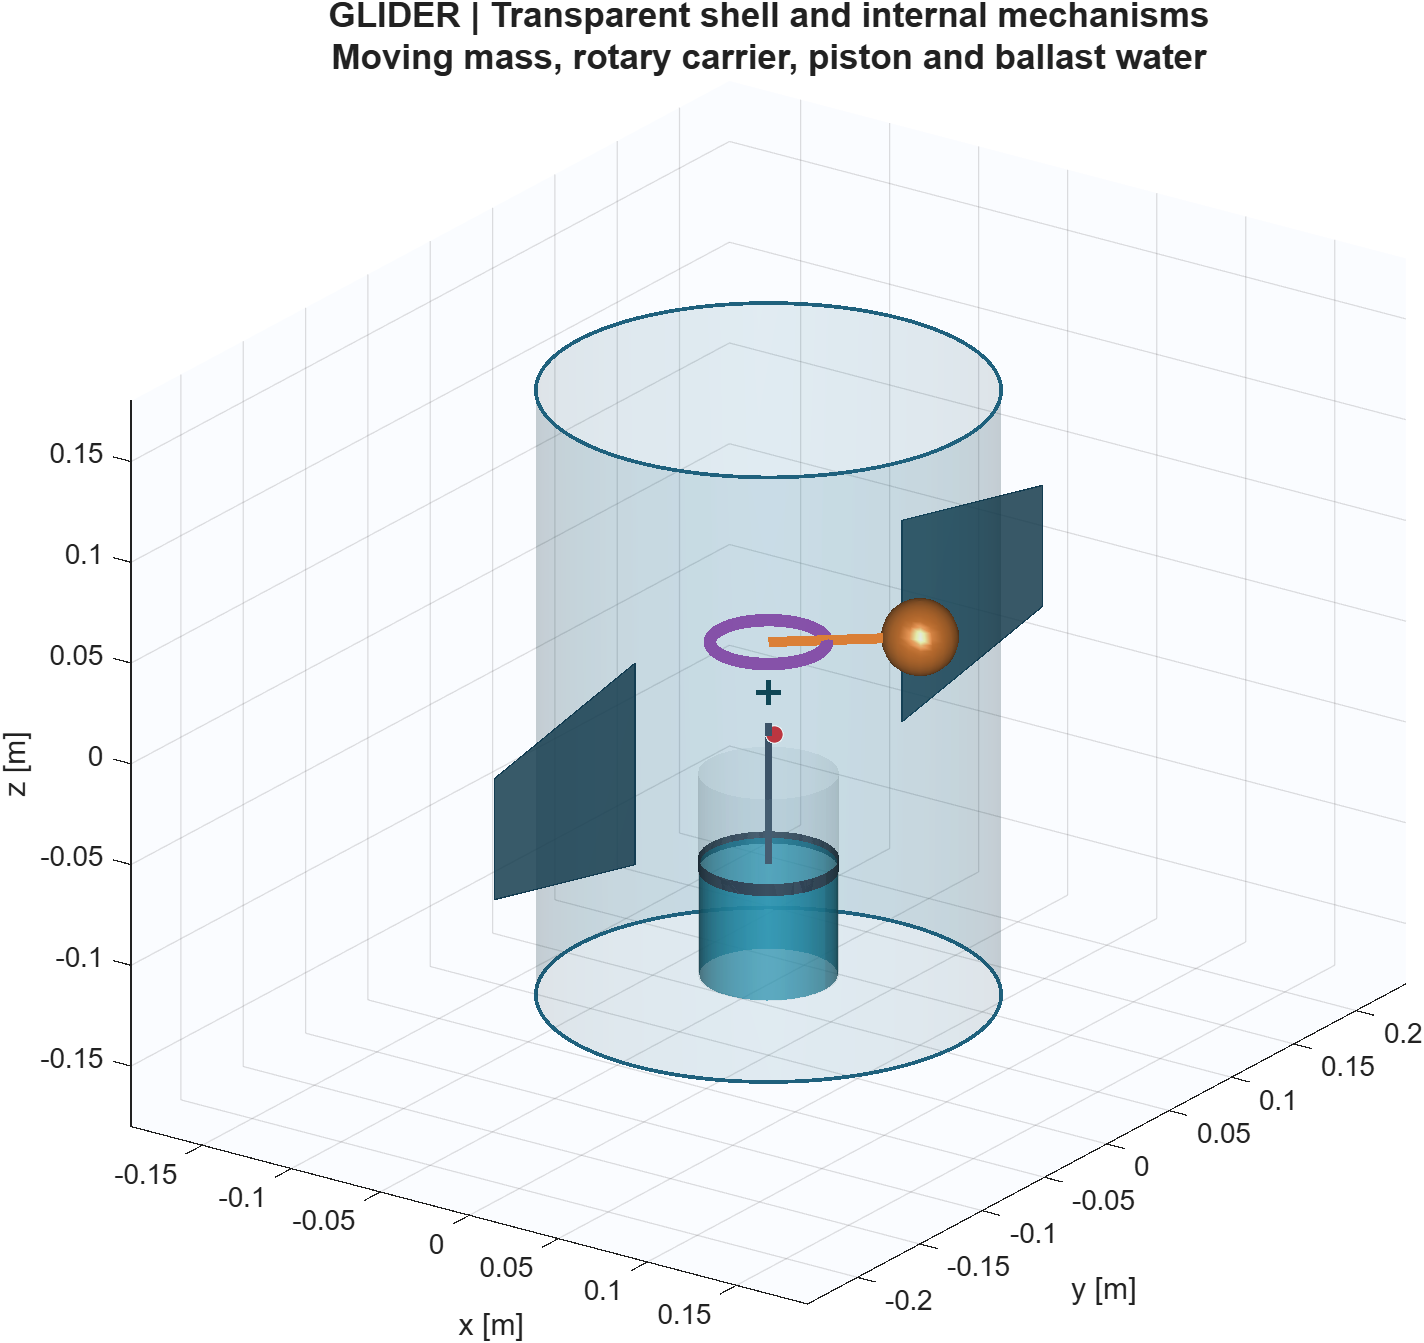
\includegraphics[width=.88\textwidth]{glider_preview.png}
\vfill
\textbf{Mechanism:} a free base, a revolute--prismatic branch and a prismatic
branch, with all joints enclosed by the hull.\\
\textbf{Scope:} an executable research model with explicitly identified
demonstration parameters. Numerical verification does not establish
experimental calibration.\\[4mm]
Johnny Garcia and Julio \hfill October 26, 2026
\end{titlepage}
\hypersetup{pageanchor=true}
\tableofcontents\clearpage

\section{Physical system and conventions}
The hull is body 1 and encloses bodies 2, 3 and 4. One branch rotates a
carrier and translates a mass; the other moves a syringe piston. Admitted
water changes the total mass, its first moment and its inertia. The
external displaced volume \(\mathcal V\) remains constant. Hydrostatic
buoyancy acts on the hull and is not assigned again to each internal body.
\begin{center}
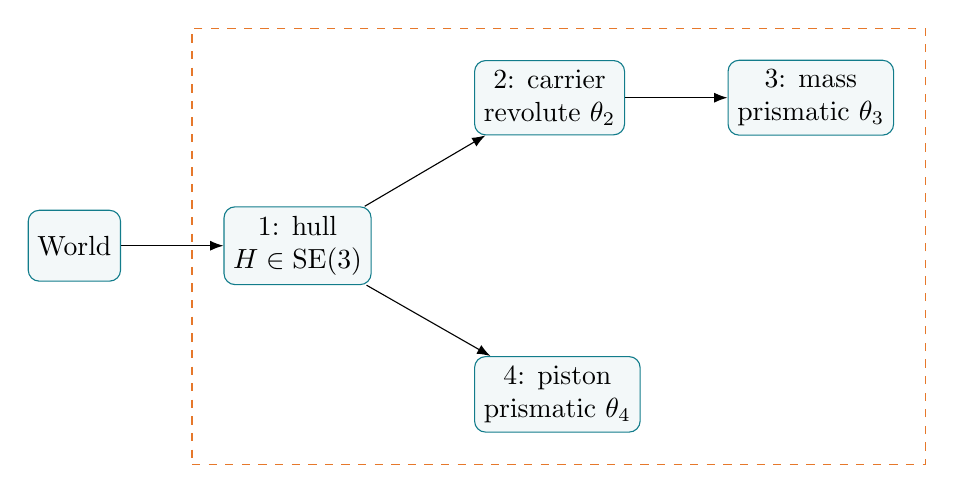
\begin{tikzpicture}[node distance=9mm and 13mm,>=Latex,
 b/.style={draw=teal,rounded corners,fill=teal!5,minimum height=9mm,align=center}]
\node[b] (world) {World};
\node[b,right=of world] (base) {1: hull\\\(H\in\SE\)};
\node[b,above right=of base] (r) {2: carrier\\revolute \(\theta_2\)};
\node[b,right=of r] (mass) {3: mass\\prismatic \(\theta_3\)};
\node[b,below right=of base] (piston) {4: piston\\prismatic \(\theta_4\)};
\draw[->] (world)--(base);\draw[->] (base)--(r);
\draw[->] (r)--(mass);\draw[->] (base)--(piston);
\node[draw=orange,dashed,fit=(base)(r)(mass)(piston),inner sep=4mm] {};
\end{tikzpicture}
\end{center}
The model assumes still exterior water, uniform density, full submergence,
rigid solids and no contact. Interior water is approximated by a
distribution sharing the rigid velocity of the hull. Its relative
circulation momentum is neglected, while momentum transport through the
port is retained explicitly. The geometric center of the water is not
treated as a material link.

The moving-mass and ballast models of Leonard and Graver motivate this
physical separation \cite{graver,leonard}. The spatial formulation of the
solids adopts the angular-first convention of Modern Robotics \cite{mr}.
Exterior-fluid added inertia is separated from dissipative forces, as in
the structure of Fossen's marine craft model \cite{fossen}.

The world \(z\)-axis points upward, with \(g_0=(0,0,-g)^\top\). The nominal
longitudinal hull axis is \(z_B\), retaining the supplied code's axis
orientation. The NED convention is not used.

\begin{tabularx}{\textwidth}{@{}lX@{}}\toprule
Symbol & Definition\\\midrule
\(H={}^{0}H_1=[R,p;0,1]\) & Pose mapping base coordinates to world coordinates.\\
\(q=(\theta_2,\theta_3,\theta_4)^\top\) & Internal coordinates, in radians and meters.\\
\(V=(\omega^\top,v^\top)^\top\in\R^6\) & Base twist expressed in the base frame.\\
\(\nu=(V^\top,\dot q^\top)^\top\in\R^9\) & Generalized velocity, not nine Cartesian coordinate derivatives.\\
\(W=(n^\top,f^\top)^\top\) & Wrench, moment first; power is \(V^\top W\).\\
\(\E=[I_6\ \ 0],\ \B=[0\ \ I_3]\) & Selectors: \(V=\E\nu\), \(\dot q=\B\nu\).\\\bottomrule
\end{tabularx}
The configuration space is \(\SE\times S^1\times\R^2\), restricted by
physical travel limits. The angle is unwrapped within \([-\pi,\pi]\).
Crossing a limit stops the simulation without representing an impact.
\clearpage

\section{Geometric tree kinematics}
For \(x\in\R^3\), let \(\sk{x}y=x\times y\). In angular-first order,
\begin{equation}
\widehat V=\begin{bmatrix}\sk{\omega}&v\\0&0\end{bmatrix},\quad
\Ad_H=\begin{bmatrix}R&0\\\sk{p}R&R\end{bmatrix},\quad
\ad_V=\begin{bmatrix}\sk{\omega}&0\\\sk{v}&\sk{\omega}\end{bmatrix}.
\end{equation}
The base satisfies \(\dot H=H\widehat V\), allowing updates through the
group exponential. The parents are \(a(2)=1\), \(a(3)=2\), \(a(4)=1\).
The constant body screw axes are
\begin{equation}
S_2=(0,0,1,0,0,0)^\top,\quad S_3=(0,0,0,1,0,0)^\top,\quad
S_4=(0,0,0,0,0,-1)^\top.
\end{equation}
Relative poses and velocity transformations are
\begin{equation}
H_i={}^{a(i)}H_i(0)\exp(\widehat S_i\theta_i),\qquad X_i=\Ad_{H_i^{-1}}.
\end{equation}
Let \(V_i\) be each body's twist relative to the world, expressed in its
own frame. The recursions are
\begin{align}
V_1&=V,& V_i&=X_iV_{a(i)}+S_i\dot\theta_i,\\
\dot V_1&=\dot V,&\dot V_i&=X_i\dot V_{a(i)}+S_i\ddot\theta_i
-\ad_{S_i\dot\theta_i}X_iV_{a(i)}.\label{eq:acc}
\end{align}
The Jacobians \(J_i\in\R^{6\times9}\) and bias accelerations \(a_i^0\)
are computed together:
\begin{equation}
V_i=J_i\nu,\qquad \dot V_i=J_i\dot\nu+a_i^0,\qquad
J=\begin{bmatrix}I&0&0&0\\X_2&S_2&0&0\\X_3X_2&X_3S_2&S_3&0\\X_4&0&0&S_4\end{bmatrix}.
\label{eq:J}
\end{equation}
The revolute column for body 3 is \(X_3S_2\), expressed in body 3.

\subsection{Equivalent matrix form}
Define
\begin{equation}
A=\begin{bmatrix}0&0&0&0\\X_2&0&0&0\\0&X_3&0&0\\X_4&0&0&0\end{bmatrix},\quad
L=(I-A)^{-1},\quad \mathsf S=\diag(I_6,S_2,S_3,S_4).
\end{equation}
The rectangular matrix \(\mathsf S\) has size \(24\times9\), and
\begin{equation}
J=L\mathsf S,\quad a^0=-LDAJ\nu,\quad
D=\diag(0_6,\ad_{S_2\dot\theta_2},\ad_{S_3\dot\theta_3},\ad_{S_4\dot\theta_4}).
\label{eq:D}
\end{equation}
The blocks of \(D\) lie on its diagonal. The recursive implementation
avoids constructing or inverting the \(24\times24\) stacked matrices.
\clearpage

\section{Inertia, gravity and buoyancy}
For mass \(m_i>0\), center of mass \(c_i\) expressed in the body frame,
and central rotational inertia \(J_{c,i}\), the spatial inertia is
\begin{equation}
\mathcal I_i=\begin{bmatrix}J_{c,i}-m_i\sk{c_i}^2&m_i\sk{c_i}\\
-m_i\sk{c_i}&m_iI_3\end{bmatrix}.\label{eq:spatial}
\end{equation}
If \(V_b=XV_a\), preservation of kinetic energy requires
\(\mathcal I_a=X^\top\mathcal I_bX\). A frame change transforms the
complete inertia matrix through this congruence. The inertial wrench is
\begin{equation}
W_i^{\rm in}=\mathcal I_i\dot V_i-\ad_{V_i}^\top\mathcal I_iV_i.
\end{equation}
With \(R_i={}^{0}R_i\), gravity and its generalized projection are
\begin{equation}
f_{g,i}=m_iR_i^\top g_0,\quad W_{g,i}=\begin{bmatrix}c_i\times f_{g,i}\\f_{g,i}\end{bmatrix},
\qquad Q_{g,d}=\sum_{i=1}^4J_i^\top W_{g,i}.\label{eq:gravity}
\end{equation}
All nine projected components are retained, including the joint
components. Gravity and inertia use the same center-of-mass locations.

For center of buoyancy \(c_B\) expressed in the base,
\begin{equation}
f_B=-\rho\mathcal V R^\top g_0,\qquad
W_B=\begin{bmatrix}c_B\times f_B\\f_B\end{bmatrix}.\label{eq:buoy}
\end{equation}
The minus sign produces an upward force using the same gravity vector
throughout the derivation. Its projection is \(\E^\top W_B\).

\subsection{Center of mass and density}
Let \(r_i(q)\) denote each solid's center of mass in the base frame.
For stored water mass \(m_w\) and center \(c_w\),
\begin{equation}
m_{\rm tot}=\sum_i m_i+m_w,\qquad
c_G(q)=\frac{\sum_i m_ir_i(q)+m_wc_w}{m_{\rm tot}}.
\end{equation}
The mean density is \(m_{\rm tot}/\mathcal V\). Moving internal masses
changes the center of mass and inertial couplings; pumping water also
changes the total mass. Neutral buoyancy requires
\(m_{\rm tot}=\rho\mathcal V\).

\subsection{Physical admissibility}
The model constructor checks symmetry, positive definiteness and the
triangle inequalities for each central inertia:
\begin{equation}
\lambda_{\max}(J_c)\leq\tfrac12\operatorname{tr}(J_c).
\end{equation}
A positive spatial matrix alone does not guarantee a physically
realizable mass distribution. The supplied hull inertia violates this
condition and is replaced by an explicitly provisional equivalent
cylinder.
\clearpage

\section{Stored water: geometry and variable inertia}
The supplied code's convention is adopted: \(0\leq\theta_4\leq\ell\),
\(\ell=0.1\,\mathrm m\), with the piston moving along \(-z_B\).
\begin{equation}
h=\ell-\theta_4,\quad A_s=\pi r_s^2,\quad m_w=\rho A_sh,\quad
\dot m_w=-\rho A_s\dot\theta_4.\label{eq:mass}
\end{equation}
The chamber is full at \(\theta_4=0\) and empty at \(\theta_4=\ell\).
For a fixed lower end \(r_t\) and \(e_3=(0,0,1)^\top\),
\begin{equation}
r_p=r_t+he_3,\qquad c_w=r_t+\tfrac12he_3.
\end{equation}
A prime denotes differentiation with respect to \(\theta_4\):
\(r_p'=-e_3\) and \(c_w'=-e_3/2\). Thus the geometric water center
does not move with the piston. Frame 4 remains attached to the dry piston.
For a uniformly filled cylinder,
\begin{equation}
J_{c,w}=\frac{m_w}{12}\diag(3r_s^2+h^2,3r_s^2+h^2,6r_s^2),\qquad
\mathcal I_w=\mathcal I(m_w,c_w,J_{c,w}).
\end{equation}
Let \(k=\rho A_s\), \(C=\sk{c_w}\), \(C'=\sk{-e_3/2}\), \(m_w'=-k\).
\begin{align}
J_{c,w}'={}&-\frac{k}{12}\diag(3r_s^2+h^2,3r_s^2+h^2,6r_s^2)
+\frac{m_w}{12}\diag(-2h,-2h,0),\\
\mathcal I_w'={}&\begin{bmatrix}
J_{c,w}'-m_w'C^2-m_w(C'C+CC')&m_w'C+m_wC'\\
-m_w'C-m_wC'&m_w'I_3\end{bmatrix},\\
\dot{\mathcal I}_w={}&\mathcal I_w'\dot\theta_4.\label{eq:Idot}
\end{align}
At empty fill, \(m_w=0\) and \(\mathcal I_w=0\), without singularities.
The water cylinder's rotational inertia is retained rather than replacing
the stored volume by a point mass.

\subsection{Interior-flow approximation}
The occupied domain changes. The velocity of its geometric center does
not determine particle velocities. In general,
\begin{equation}
p_w=\mathcal I_wV+p_{\rm rel},\qquad
p_{\rm rel}=\int_{\Omega_w}\begin{bmatrix}r\times u_{\rm rel}(r)\\u_{\rm rel}(r)\end{bmatrix}\,dm.
\end{equation}
The implemented closure takes \(p_{\rm rel}\simeq0\). This must be
revisited when circulation, flow rate, sloshing or pipe flow produces
appreciable relative momentum. A fill-dependent inertia alone then
cannot replace an interior-flow model.
\clearpage

\section{Open-system momentum balance}
The momentum expressed in the base and referred to its origin is
\begin{equation}
P_B=\sum_i\Ad_{{}^{1}H_i^{-1}}^\top\mathcal I_iV_i+\mathcal I_wV+M_AV.
\end{equation}
Here \(M_A\) is a constant, symmetric positive-semidefinite added
hydrodynamic inertia of the exterior water; it is distinct from stored
ballast water. For a control volume admitting or expelling water,
\begin{equation}
\dot P_B-\ad_V^\top P_B=W_{\rm ext}+\Phi,\qquad
\Phi=\dot m_w\begin{bmatrix}r_o\times u_o\\u_o\end{bmatrix}.\label{eq:flux}
\end{equation}
The effective port location is \(r_o\), and \(u_o\) is the absolute
transport velocity expressed in the base. The demonstration closure,
without a resolved directional jet, is
\begin{equation}
u_o=\begin{cases}0,&\dot m_w\geq0\quad\text{(inflow from still water)},\\
v+\omega\times r_o,&\dot m_w<0\quad\text{(comoving outflow)}.\end{cases}
\end{equation}
A real jet requires a consistent addition of relative velocity and
pressure forces. Exterior current also requires changes to hydrodynamic
forces and relative added-inertia dynamics. The option
\texttt{water.flux='zero'} selects an alternative idealization of zero
net momentum transport, requiring its own physical justification.

The stored-water inertial contribution is
\begin{equation}
\boxed{\mathcal I_w\dot V+\dot{\mathcal I}_wV-\ad_V^\top\mathcal I_wV.}
\label{eq:waterbalance}
\end{equation}
The inertia derivative has a positive sign on the inertial side;
\(\Phi\) is on the force side. Subtracting an inertia derivative from
\(\ad_V\) would combine objects of different physical dimensions and
does not represent this balance.

\subsection{Translational sign check}
For a point mass without rotation,
\begin{equation}
m\dot v+\dot m\,v=F+\dot m\,u_o.
\end{equation}
During admission of still water, \(u_o=0\): the vehicle accelerates
the mass it acquires. During comoving expulsion, \(u_o=v\), and the
two \(\dot m\,v\) terms cancel. Omitting flux cannot represent both
processes indiscriminately.

The water contributes the gravity wrench
\begin{equation}
W_{g,w}=\begin{bmatrix}c_w\times(m_wR^\top g_0)\\m_wR^\top g_0\end{bmatrix},
\end{equation}
which enters the base rows under this closure. The hydraulic piston
load is specified separately.
\clearpage

\section{Hull, wings and syringe load}
At a load center \(r_H\), let \(v_H=v+\omega\times r_H\),
\(s=\|v_H\|\), \(e=v_H/s\), with unit wing normal \(n\) and unit lateral
direction \(b_s\). For \(s>0\), the demonstration force model is
\begin{align}
f_L&=-k_Ls(n^\top v_H)\bigl[n-(n^\top e)e\bigr],\\
f_D&=-[k_D+k_{D\alpha}(n^\top e)^2]s\,v_H
-k_s|b_s^\top v_H|(b_s^\top v_H)b_s,\\
n_D&=-d_\omega\odot\omega-k_\omega\odot|\omega|\odot\omega,\\
W_H&=\begin{bmatrix}r_H\times(f_L+f_D)+n_D\\f_L+f_D\end{bmatrix}.\label{eq:hydro}
\end{align}
At zero speed, \(f_L=f_D=0\). Dissipation coefficients are nonnegative.
The coefficients \(k_L,k_D,k_{D\alpha},k_s\) have units
\(\mathrm{kg/m}\); rotational coefficients produce \(n_D\) in
\(\mathrm{N\,m}\). The power identities are
\begin{equation}
v_H^\top f_L=0,\qquad V^\top W_H=v_H^\top f_D+\omega^\top n_D\leq0.
\end{equation}
They hold for reversed flow as well. Lift contributes no instantaneous
power. This force surrogate has neither experimental identification nor
a stall model. Added inertia contributes
\(M_A\dot V-\ad_V^\top M_AV\). Fossen's linear-first matrices must be
permuted before use with this project's angular-first convention.

\subsection{Quasistatic hydraulic load}
Pressure produces an equivalent internal piston effort:
\begin{align}
x_p&=p+Rr_p,\quad
\Delta p=p_{\rm surface}+\rho g_0^\top x_p-p_{\rm back},\\
f_p&=-A_s\Delta p-d_p\dot\theta_4-f_c\tanh(\dot\theta_4/v_s),\\
Q_p&=(0,\ldots,0,f_p)^\top\in\R^9.\label{eq:pump}
\end{align}
Exterior pressure increases with depth. For \(\Delta p>0\), the
negative load \(f_p\) opposes water expulsion, \(\dot\theta_4>0\).
The internal force and reaction cancel under a rigid variation of the
complete assembly, so \(Q_p\) has no base component.

The example uses constant
\(p_{\rm back}=p_{\rm surface}=101325\,\mathrm{Pa}\), with \(d_p=f_c=0\).
This is a constant-back-pressure assumption. A sealed gas chamber
requires a pressure--volume law; valves, seals, pipe losses and
efficiencies require further data. Setting \texttt{pump.enabled=false}
disables this equivalent load.
\clearpage

\section{Complete equations and adapted RNEA}
The dry-body contribution is
\begin{align}
M_d&=\sum_iJ_i^\top\mathcal I_iJ_i,\\
b_d&=\sum_iJ_i^\top(\mathcal I_i a_i^0-\ad_{V_i}^\top\mathcal I_iV_i).
\end{align}
The implemented system is
\begin{equation}
\boxed{M(q)\dot\nu+b(q,\nu)=\B^\top\tau+Q(H,q,\nu),}\label{eq:main}
\end{equation}
where
\begin{align}
M&=M_d+\E^\top(\mathcal I_w+M_A)\E,\\
b&=b_d+\E^\top[\dot{\mathcal I}_wV-\ad_V^\top(\mathcal I_w+M_A)V],\\
Q&=Q_{g,d}+\E^\top(W_{g,w}+W_B+W_H+\Phi)+Q_p.
\end{align}
Actuation \(\tau\in\R^3\) contains one torque and two forces. The base
has no direct actuation, while external loads act on it. For constant
solid-body inertias, an equivalent matrix expression is
\begin{equation}
C_d\nu=J^\top[-\mathcal I LDA-\ad_{\mathcal V}^\top\mathcal I]J\nu,
\end{equation}
with \(\mathcal V=J\nu\), \(\mathcal I=\diag(\mathcal I_1,\ldots,\mathcal I_4)\)
and \(\ad_{\mathcal V}=\diag(\ad_{V_1},\ldots,\ad_{V_4})\).
Simulation needs the bias vector \(b\); a unique Coriolis matrix need
not be selected.

\subsection{Recursive Newton--Euler passes}
The forward pass obtains \(V_i,\dot V_i\) using \eqref{eq:acc} and
initializes
\begin{equation}
F_i=\mathcal I_i\dot V_i-\ad_{V_i}^\top\mathcal I_iV_i-W_{g,i}.
\end{equation}
At the root, add
\begin{equation}
(\mathcal I_w+M_A)\dot V+\dot{\mathcal I}_wV
-\ad_V^\top(\mathcal I_w+M_A)V-W_{g,w}-W_B-W_H-\Phi.
\end{equation}
The backward pass processes bodies \(4,3,2\):
\begin{equation}
\tau_i^*=S_i^\top F_i,\qquad F_{a(i)}\leftarrow F_{a(i)}+X_i^\top F_i.
\end{equation}
Subtract \(Q_p\) from \((F_1,\tau_2^*,\tau_3^*,\tau_4^*)\). The resulting
vector equals \(M\dot\nu+b-Q\). Its base block is the wrench required
by the requested acceleration and must vanish for a realizable
unactuated-base acceleration.

The function \texttt{inverse\_dynamics.m} executes this backward pass
without calling the matrix assembly. The equivalence test checks both
routes independently while sharing the kinematic formulation.
\clearpage

\section{Simulation and integration on the group}
\subsection{Prescribed-joint mode}
Given \(q,\dot q,\ddot q\), partition the equations into base and joint
blocks:
\begin{align}
\dot V&=M_{bb}^{-1}(Q_b-b_b-M_{bq}\ddot q),\\
\tau&=M_{qb}\dot V+M_{qq}\ddot q+b_q-Q_q.
\end{align}
The implementation solves a linear system with backslash rather than
forming an inverse. RNEA recovers the reactions. Sufficient actuation
is assumed; a prescribed reference does not establish that a particular
motor can realize it.

\subsection{Effort-driven mode}
For \(\tau=\tau(t,H,q,\nu)\), solve
\begin{equation}
\dot\nu=M^{-1}(\B^\top\tau+Q-b),\qquad
\dot q=\B\nu,\qquad \dot H=H\widehat{\E\nu}.
\end{equation}
A callback can supply a controller. Travel limits stop integration;
hard stops and impacts are not modeled.

\subsection{Geometric midpoint method}
Let \(f(t,H,q,\nu)\) be the acceleration of the selected mode. For
step \(\Delta t\), with \(a_n=\dot\nu_n\),
\begin{align}
H_{1/2}&=H_n\exp(\tfrac{\Delta t}{2}\widehat V_n),&
\nu_{1/2}&=\nu_n+\tfrac{\Delta t}{2}a_n,\\
q_{1/2}&=q_n+\tfrac{\Delta t}{2}\dot q_n,&
a_{1/2}&=f(t_n+\tfrac{\Delta t}{2},H_{1/2},q_{1/2},\nu_{1/2}),\\
H_{n+1}&=H_n\exp(\Delta t\widehat V_{1/2}),&
\nu_{n+1}&=\nu_n+\Delta t\,a_{1/2},\\
q_{n+1}&=q_n+\Delta t\,\dot q_{1/2}.&&
\end{align}
Prescribed joint references are evaluated directly at every stage. The
method is second order for sufficiently regular dynamics and retains
\(H\in\SE\) up to roundoff. It is neither exactly energy preserving nor
a variational integrator.

The exponential uses Rodrigues coefficients and the translation
Jacobian, with series near zero angle. It is checked against
\texttt{expm}. The simulated pose is not integrated through Euler angles
or projected afterward to repair orthogonality. The graphics transform
alone is reconstructed to satisfy the renderer's numerical tolerances.

\subsection{Example maneuver}
Each transition uses \(s(u)=10u^3-15u^4+6u^5\), \(0\leq u\leq1\), with
analytic derivatives. The example alternates \(\theta_4=0.015\) and
\(0.095\,\mathrm m\), holds \(\theta_3=0.030\,\mathrm m\), and rotates
the mass through \(0,\pi,0,-\pi,0\). Transitions last four seconds,
with sixteen-second constant segments.
\clearpage

\section{Open-system energy balance}
The mechanical energy stored by the reduced model is
\begin{align}
K&=\tfrac12\nu^\top M\nu,\\
U&=-\sum_i m_ig_0^\top(p+Rr_i)-m_wg_0^\top(p+Rc_w)
+\rho\mathcal V g_0^\top(p+Rc_B),\\
E&=K+U.
\end{align}
Let \(s_w=m_wc_w\) be the water's first moment in the base. The balance is
\begin{equation}
\boxed{\dot E=\tau^\top\dot q+V^\top W_H+\nu^\top Q_p+P_{\rm open},}
\end{equation}
where
\begin{equation}
P_{\rm open}=V^\top\Phi-\tfrac12V^\top\dot{\mathcal I}_wV
-g_0^\top(\dot m_wp+R\dot s_w).\label{eq:energyopen}
\end{equation}
Multiplying \eqref{eq:main} by \(\nu^\top\), the dry contribution satisfies
\(\nu^\top b_d=\frac12\nu^\top\dot M_d\nu\). Coadjoint terms contribute
no power. The derivative of \(K\) contains
\(\frac12V^\top\dot{\mathcal I}_wV\), whereas the bias contains
\(V^\top\dot{\mathcal I}_wV\). Their difference gives the sign in
\eqref{eq:energyopen}. Conservative forces cancel the rigid-motion part
of \(\dot U\); changes in mass and first moment leave the final term.

At fixed fill, with no hydraulic load or dissipation,
\(\dot E=\tau^\top\dot q\). Pumping makes this an open system, so constant
\(E\) is not expected. Four power channels are logged: actuation,
hydrodynamics, transport and storage change, and hydraulic loading.

\subsection{Physical interpretation and scope}
The term \(\nu^\top Q_p\) represents work exchanged with the fluid and
rear chamber under the pressure closure. Gas internal energy and
electrical losses are not included in \(E\). Joint efforts alone do
not determine electrical consumption. Transported potential power
depends on the potential datum, as expected when mass crosses the
control boundary.

Verification compares Jacobians with pose differences, inertia and bias
with Euler--Poincar\'e/Lagrange calculations, gravity with potential
derivatives, and RNEA with the matrix equations. It also checks mass flux,
pressure signs and the instantaneous energy balance. Without external
forces and with fixed ballast, the spatial momentum
\(\Ad_{H^{-1}}^\top P_B\) converges to a constant as the step is refined.
A norm combining angular and linear momentum is a mixed-unit numerical
indicator, not a universal physical error bound.
\clearpage

\section{Parameters and provenance}
\begin{tabularx}{\textwidth}{@{}l l X@{}}\toprule
Quantity & Value & Treatment\\\midrule
\(\rho,g\) & \(1000;\ 9.8\) & Supplied code, SI units.\\
Diameter and length & \(0.2142;\ 0.300\) m & Nominal code dimensions.\\
Dry masses & \(10.780;\ .50003;\ .50003;\ .150\) kg & Retained.\\
Displaced mass & \(12.096\) kg & Effective volume \(0.012096\,\mathrm{m^3}\).\\
Syringe & \(d_s=.065,\ \ell=.100\) m & Supplied-code convention.\\
Travel limits & \(\pm\pi;\ [0,.04];\ [0,.1]\) & Retained, radians and meters.\\
Dry center of body 1 & \((0,0,-.0225)\) m & Supplied gravity offset.\\
Inertias of 2, 3, 4 & See \texttt{parameters.m} & Retained diagonal tensors.\\
Central inertia of 1 & Equivalent cylinder & Admissible provisional replacement.\\
R mount and P guide & \((0,0,.025)\); \(.040\) m & Proposed enclosed mounting.\\
Syringe end & \((0,0,-.140)\) m & Proposed axial clearance.\\
\(M_A\) & \(\diag(.02,.02,.01,2,6,3)\) & Demonstration values: \(\mathrm{kg\,m^2}\), then kg.\\
Hydrodynamics & Equation \eqref{eq:hydro} & New, unidentified force law.\\
Back pressure & \(101325\) Pa & Constant example assumption.\\\bottomrule
\end{tabularx}

The nominal cylinder displaces approximately \(10.81\) liters, unlike
the \(12.096\)-liter effective volume used for buoyancy. Visual geometry
does not determine that volume; a measurement of the complete assembly
and appendages is still needed.

The original base inertia has \(J_z>J_x+J_y\), even before resolving
its center offset. The original moving mass can reach radius
\(0.13\,\mathrm m\), exceeding \(0.1071\,\mathrm m\). The proposed layout
leaves \(9.1\) mm radial clearance for the visual mass sphere over its
travel range. This is not a CAD collision check of all components.

The supplied PDF also uses \(d_s=.058\,\mathrm m\),
\(h=.10-2\theta_4\), and \(.05\,\mathrm m\) travel. That is a different
convention. This document consistently uses \eqref{eq:mass}.
The file \texttt{docs/SOURCE\_AUDIT.md} records the original locations
of discrepancies in \(D\), the Jacobian, buoyancy signs, inertia
transformation, inertia derivatives and gravity projection. Source
inputs are retained locally with hashes and excluded from distribution.
\clearpage

\section{Verification results}
% Generated from verified MATLAB JSON receipts by tools/prepare_document.py.
\newcommand{\JacError}{\(4.689\times10^{-10}\)}
\newcommand{\MassError}{\(3.290\times10^{-10}\)}
\newcommand{\RneaError}{\(3.730\times10^{-14}\)}
\newcommand{\EnergyRateError}{\(1.349\times10^{-7}\)}
\newcommand{\OrthError}{\(1.223\times10^{-14}\)}
\newcommand{\PositionError}{\(1.313\times10^{-5}\)}
\newcommand{\RotationError}{\(9.019\times10^{-5}\)}
\newcommand{\EnergyError}{\(4.479\times10^{-4}\)}
\newcommand{\FineEnergyError}{\(1.082\times10^{-4}\)}
\newcommand{\MomentumError}{\(1.184\times10^{-6}\)}
\newcommand{\FineMomentumError}{\(2.962\times10^{-7}\)}
\newcommand{\ClosedEnergyError}{\(7.678\times10^{-9}\)}
\newcommand{\FineClosedEnergyError}{\(1.920\times10^{-9}\)}
\newcommand{\DepthMin}{3.771}
\newcommand{\DepthMax}{8.251}
\newcommand{\HorizontalRange}{1.387}
\newcommand{\TauOne}{0.02809}
\newcommand{\TauTwo}{0.8399}
\newcommand{\TauThree}{271.2}

Verification used MATLAB R2026a and random seed 42. The example runs
for 80 seconds with a \(0.02\)-second step and is repeated at \(0.01\) s.
\begin{center}\begin{tabular}{@{}lr@{}}\toprule
Test or indicator & Result\\\midrule
Random states & 25\\
Maximum Jacobian error & \JacError\\
Relative inertia disagreement & \MassError\\
RNEA / matrix disagreement & \RneaError\\
Instantaneous energy-rate error & \EnergyRateError\\
Example \(\max\|R^\top R-I\|_F\) & \OrthError\\
Position difference after refinement & \PositionError\ m\\
Orientation difference after refinement & \RotationError\ rad\\
Energy residual at \(0.02\) s & \EnergyError\ J\\
Energy residual at \(0.01\) s & \FineEnergyError\ J\\\bottomrule
\end{tabular}\end{center}
Absolute disagreements combining different components are SI numerical
consistency checks. Complete values and thresholds are available in
\path{results/validation.json} and \path{tests/validate_glider.m}.

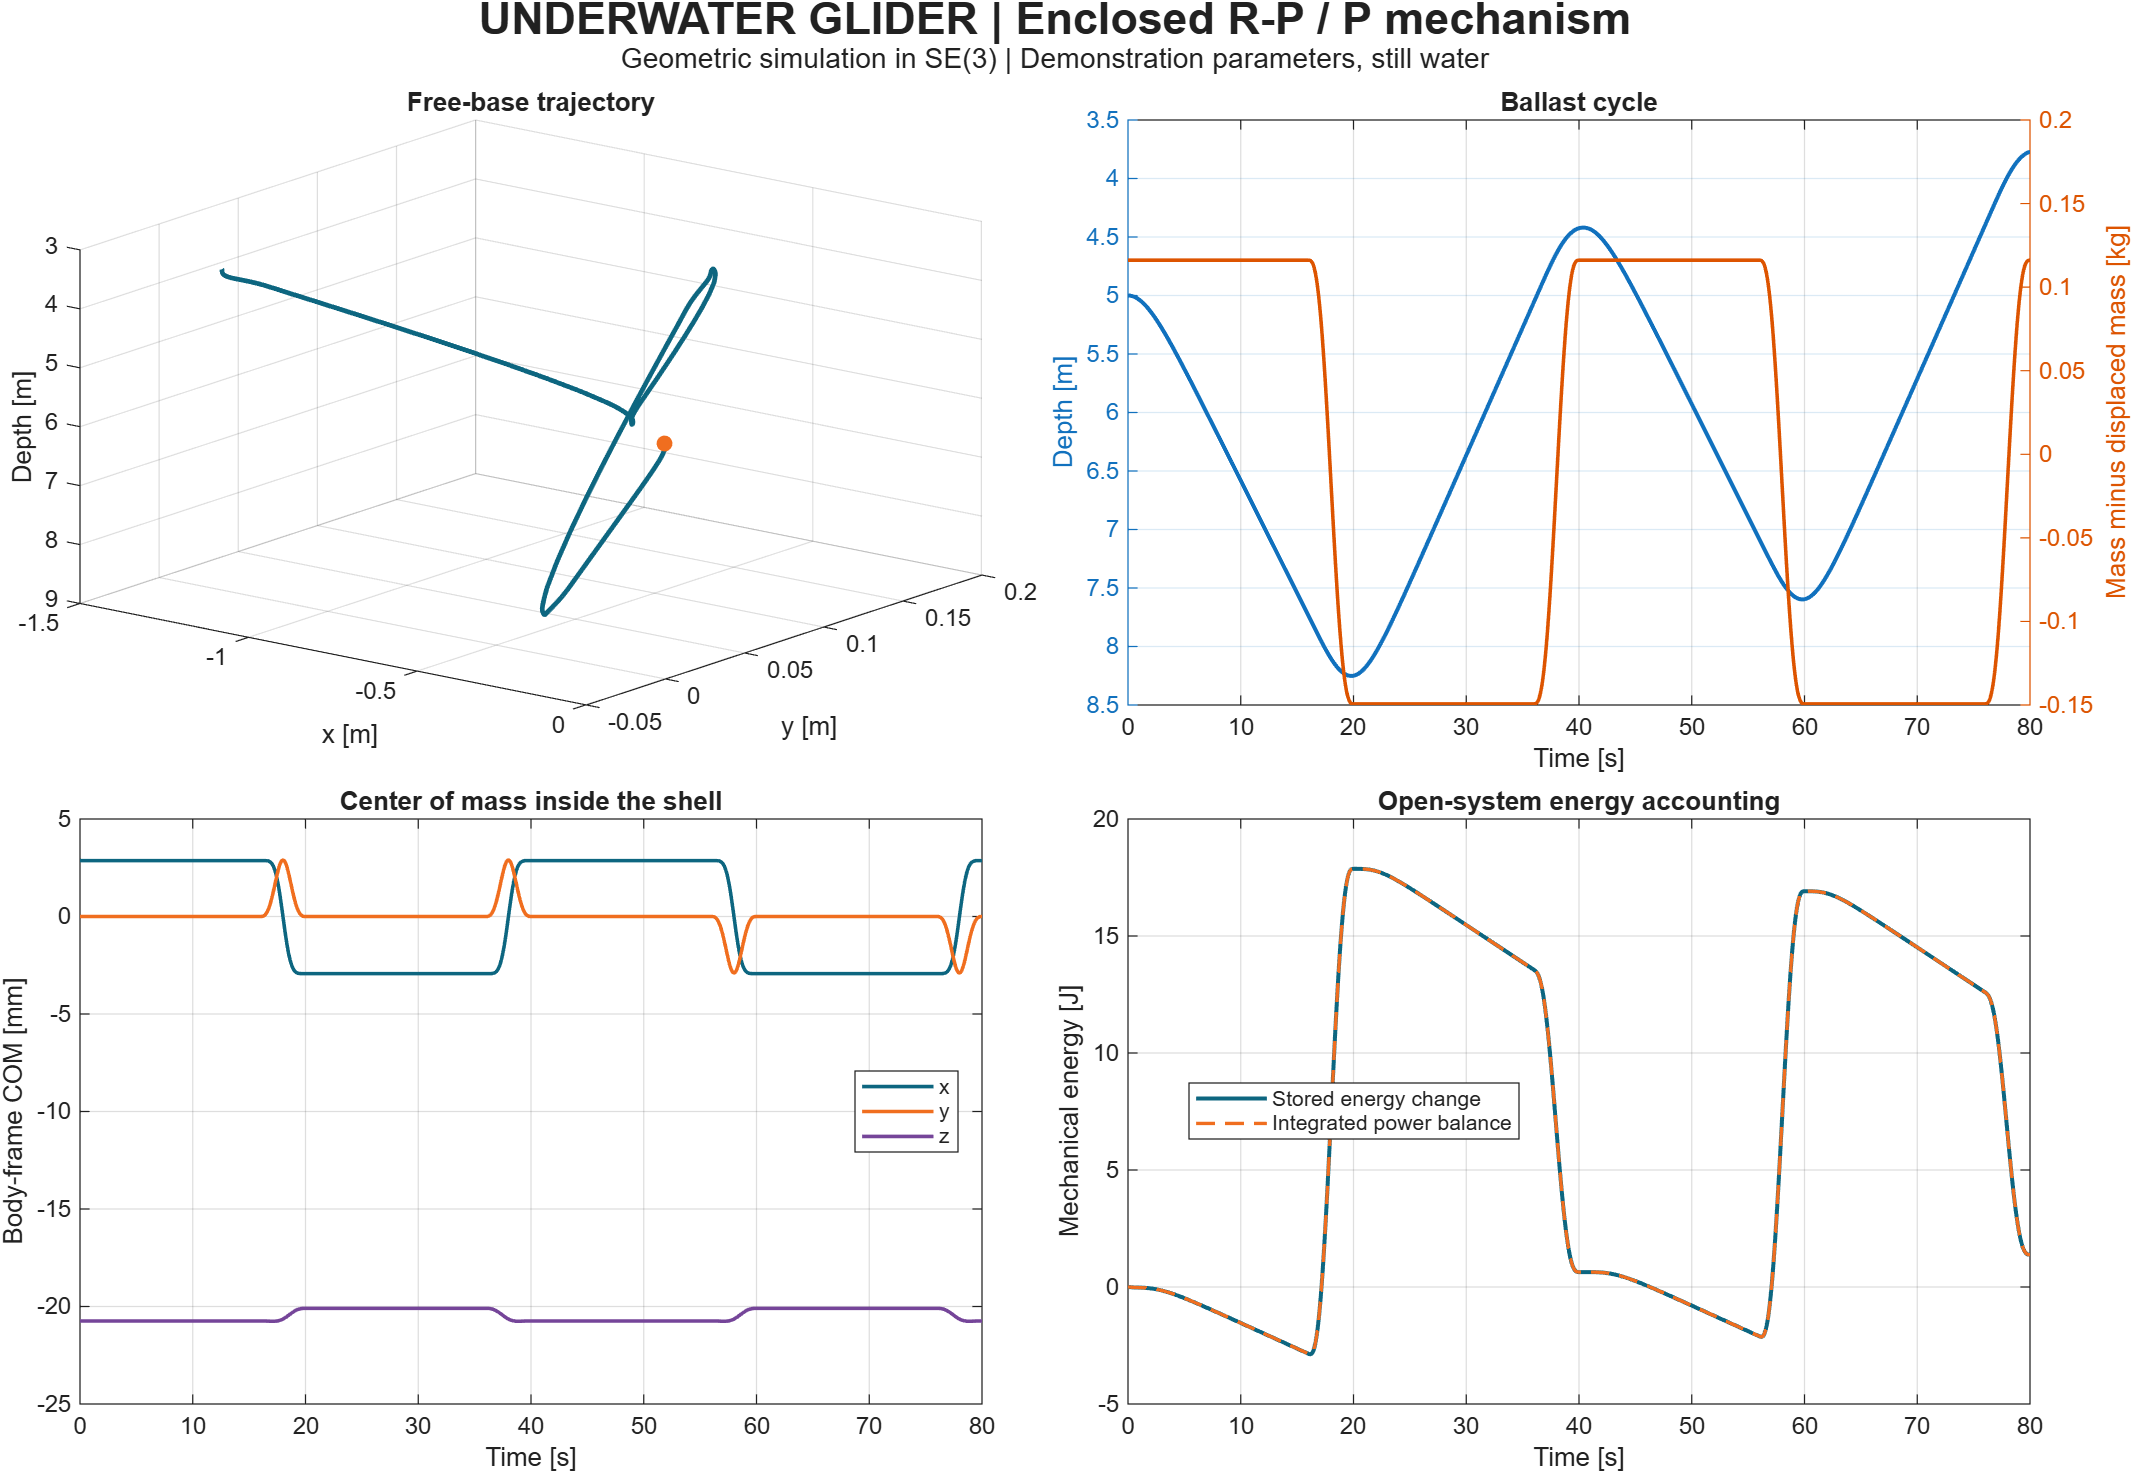
\includegraphics[width=\textwidth]{simulation.png}

Depth ranges from \DepthMin\ to \DepthMax\ m, and the maximum horizontal
displacement from the start is \HorizontalRange\ m. These are outputs
of the parameterized demonstration, not calibrated prototype predictions.
\clearpage

\subsection{Efforts and convergence}
\hspace*{.04\textwidth}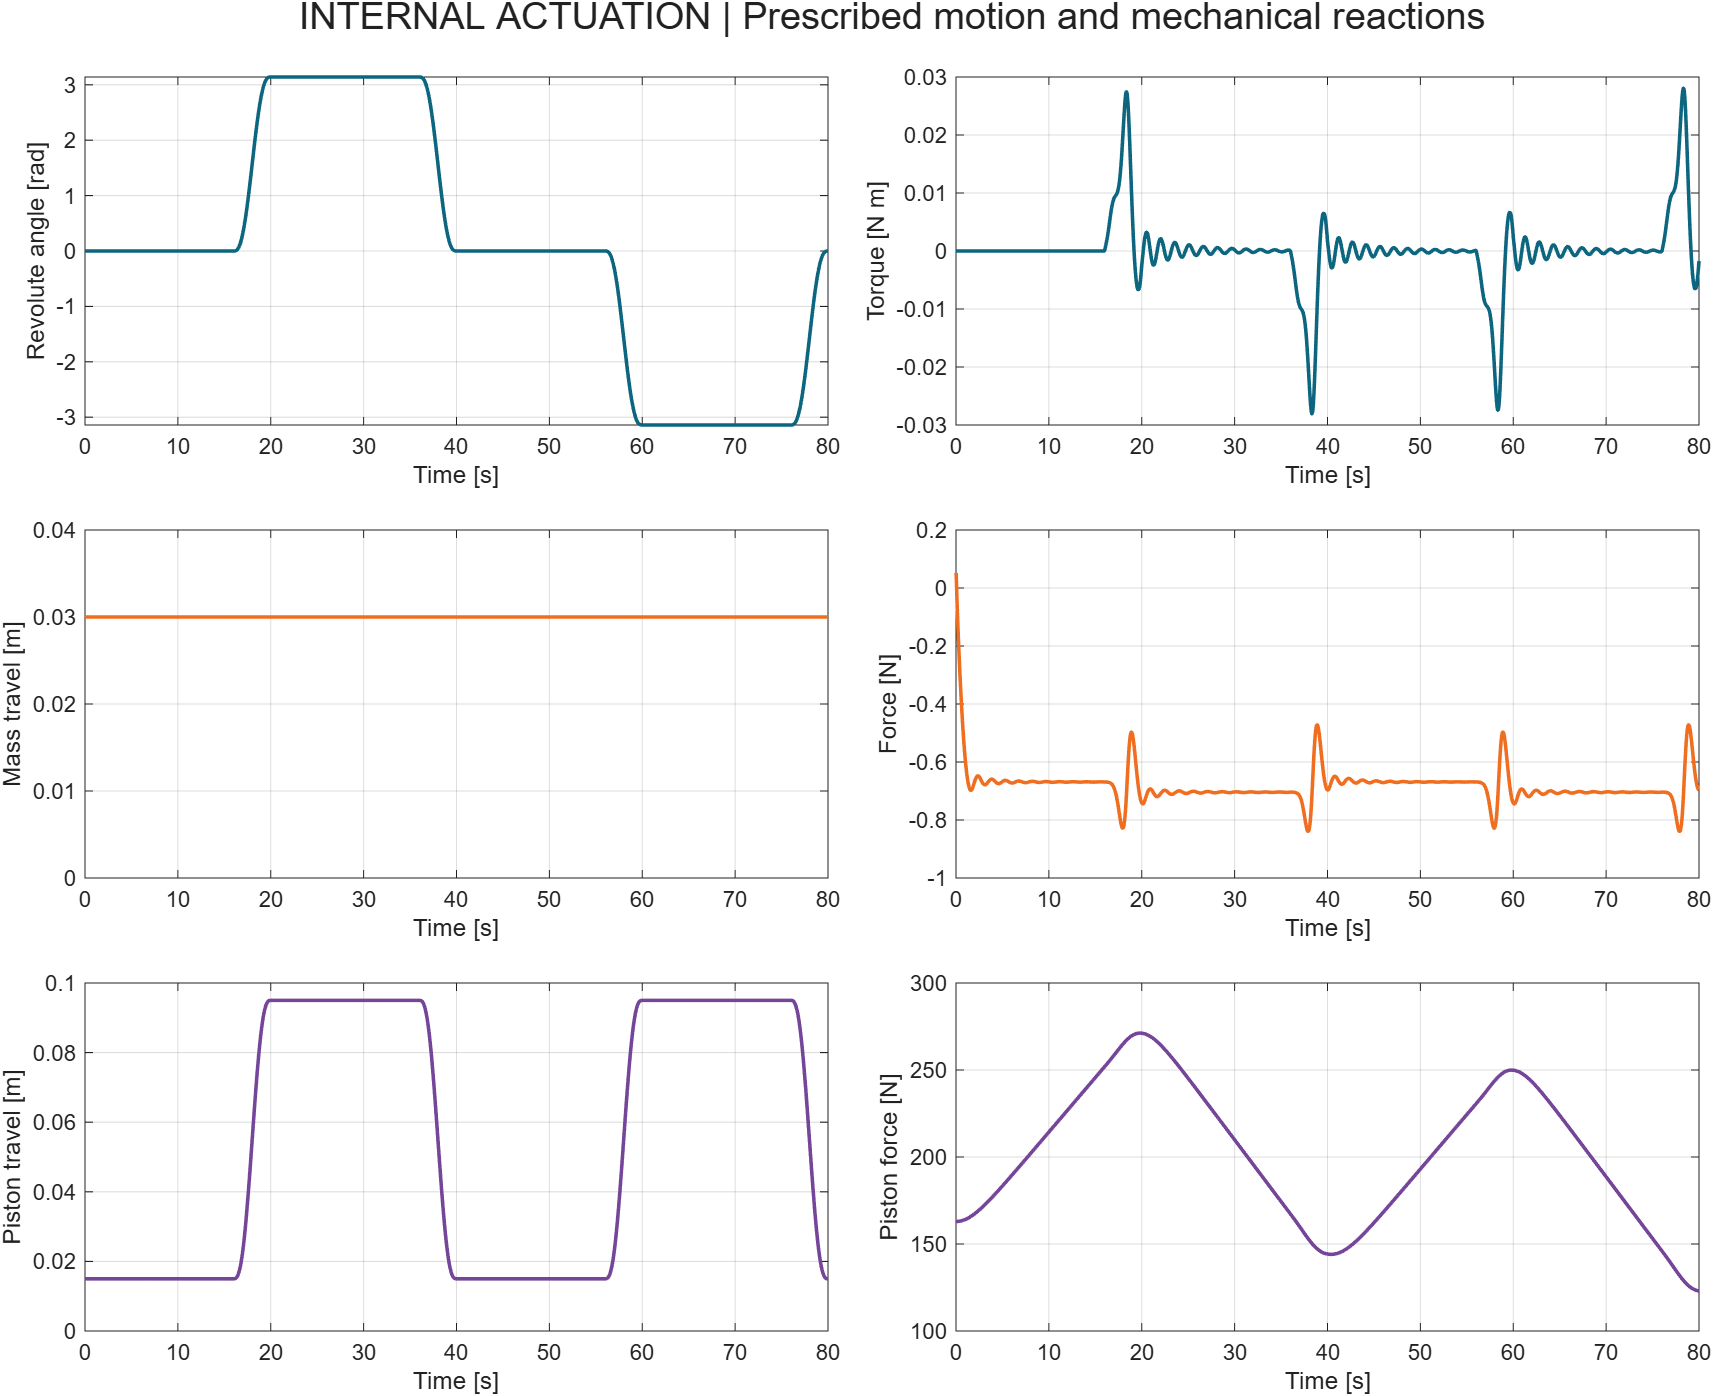
\includegraphics[width=.92\textwidth]{actuation.png}\par
Maximum absolute efforts are \TauOne\ \(\mathrm{N\,m}\), \TauTwo\ N,
and \TauThree\ N. Syringe force is dominated by pressure under the
constant-back-pressure assumption. These are unsaturated model demands,
not confirmed actuator capabilities.

\hspace*{.04\textwidth}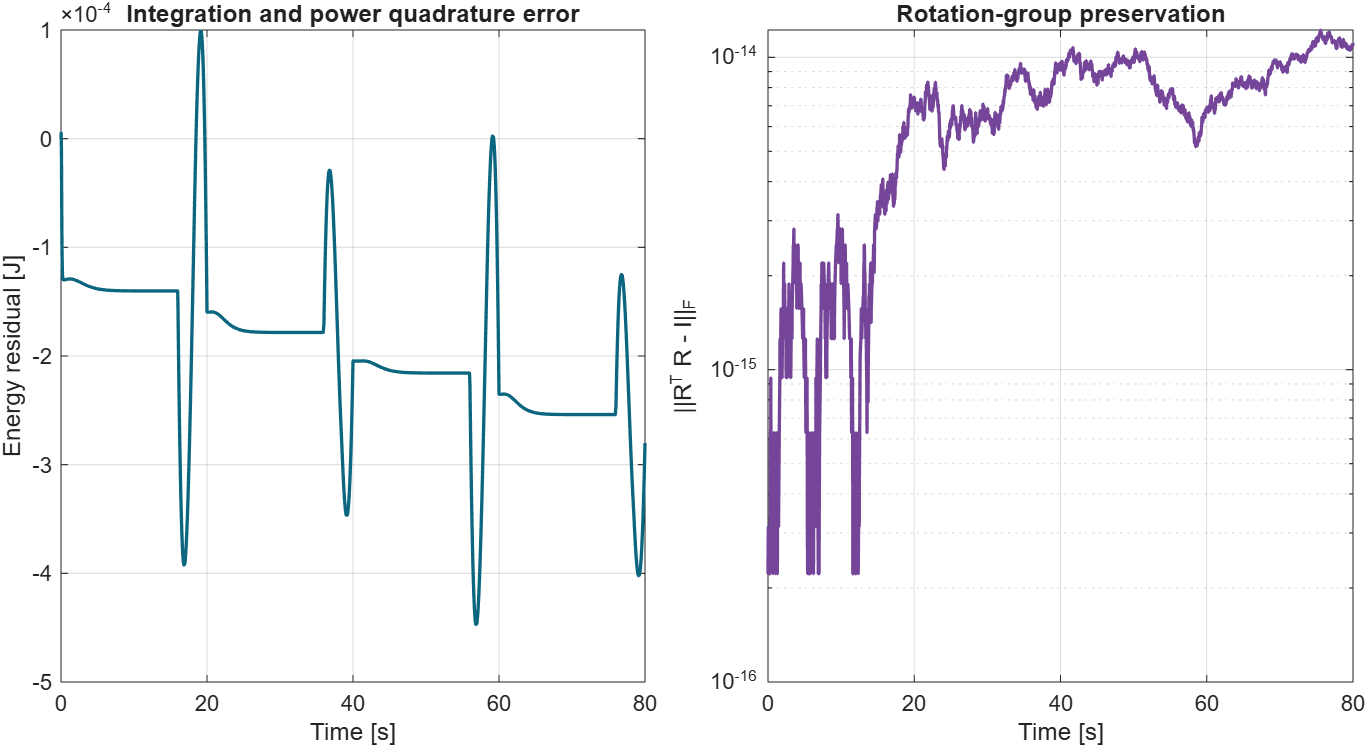
\includegraphics[width=.92\textwidth]{diagnostics.png}\par
In the isolated momentum test, reducing the step from \(0.01\) to
\(0.005\) s reduces the error from \MomentumError\ to \FineMomentumError.
The energy error falls from \ClosedEnergyError\ to \FineClosedEnergyError\ J,
consistent with second-order integration.
\clearpage

\section{Usage and code correspondence}
From the repository root:
\begin{lstlisting}
setup_glider;
summary = run_glider_demo();
addpath('tests'); validate_glider;
addpath('examples');
s = load('results/demo.mat');
animate_glider(s.log, s.m);
\end{lstlisting}
Edit parameters before constructing a new model:
\begin{lstlisting}
p = glider.parameters();
p.pump.back_pressure = 101325; % replace with the physical value
m = glider.model(p);
c = glider.config();
log = glider.simulate(m,c);
\end{lstlisting}
For effort-driven dynamics, select \texttt{c.mode='effort'} and assign
\texttt{c.effort=@(t,H,q,nu,m) ...}, returning three efforts. Start with
short horizons and a controller respecting travel and actuator limits.

\begin{tabularx}{\textwidth}{@{}lX@{}}\toprule
Function in \texttt{+glider/} & Responsibility\\\midrule
\texttt{parameters, model} & Editable data and checked constants.\\
\texttt{kinematics} & Tree recursions, equations \eqref{eq:acc}--\eqref{eq:J}.\\
\texttt{spatial\_inertia, water} & Spatial inertia and fill derivative.\\
\texttt{hydrodynamics, pump\_load} & Hull loads and piston pressure.\\
\texttt{dynamics} & Equation \eqref{eq:main}, loads and energy.\\
\texttt{inverse\_dynamics} & Branched RNEA with root corrections.\\
\texttt{hybrid\_dynamics, forward\_dynamics} & Free base with references or efforts.\\
\texttt{exp\_se3, simulate} & Integration and consistent logging.\\
\texttt{draw\_robot, plot\_results} & Procedural geometry and figures.\\\bottomrule
\end{tabularx}

\subsection{Prototype data still required}
Calibration requires CAD or measured axis and mass locations, central
inertias, displaced volume, center of buoyancy, syringe pressure and
flow rate, back pressure, losses, motor limits, and hydrodynamic
identification. These replace the demonstration parameters while
retaining the conventions and verification tests.

\begin{thebibliography}{9}
\bibitem{mr} K. M. Lynch and F. C. Park, \emph{Modern Robotics: Mechanics,
Planning, and Control}, Cambridge University Press, 2017.
\href{https://modernrobotics.northwestern.edu/nu-gm-book-resource/8-2-dynamics-of-a-single-rigid-body-part-2-of-2/}{Official material, Section 8.2}.
\bibitem{fossen} T. I. Fossen, \emph{Fossen's Marine Craft Model}.
\url{https://www.fossen.biz/html/marineCraftModel.html}.
Accessed October 26, 2026.
\bibitem{graver} J. G. Graver, \emph{Underwater Gliders: Dynamics, Control
and Design}, Ph.D. thesis, Princeton University, 2005.
\href{https://naomi.princeton.edu/wp-content/uploads/sites/744/2021/03/jggraver-thesis-4-11-05.pdf}{Full text at N. E. Leonard's laboratory}.
\bibitem{leonard} N. E. Leonard and J. G. Graver, Model-based feedback control
of autonomous underwater gliders, \emph{IEEE Journal of Oceanic Engineering},
26(4), 633--645, 2001. \url{https://doi.org/10.1109/48.972106}.
\end{thebibliography}
\end{document}
